\documentclass[12pt, a4paper]{article}

% ── Packages ──────────────────────────────────────────────────────────────────
\usepackage{amsmath, amssymb, amsthm}
\usepackage{geometry}
\usepackage{booktabs}
\usepackage{array}
\usepackage{hyperref}
\usepackage{xcolor}
\usepackage{tcolorbox}
\usepackage{enumitem}
\usepackage{parskip}
\usepackage{tikz}
\usetikzlibrary{arrows.meta, positioning, calc}

\geometry{margin=2.5cm}

% ══════════════════════════════════════════════════════════════════════════════
% ── Student-mode switch ───────────────────────────────────────────────────────
\newif\ifstudentmode
\studentmodefalse

\ifx\studentflag\undefined
\else
  \studentmodetrue
\fi
% ══════════════════════════════════════════════════════════════════════════════

% ── Student-mode macros ───────────────────────────────────────────────────────
\newcommand{\sol}[2][6cm]{%
  \ifstudentmode
    \underline{\hspace{#1}}%
  \else
    {#2}%
  \fi
}

\newcommand{\soleq}[2][3cm]{%
  \ifstudentmode
    \par\vspace{4pt}%
    \noindent\rule{\linewidth}{0.5pt}\\[#1]%
    \noindent\rule{\linewidth}{0.5pt}%
    \par\vspace{4pt}%
  \else
    \[#2\]%
  \fi
}
% ──────────────────────────────────────────────────────────────────────────────

% ── Colors & boxes ────────────────────────────────────────────────────────────
\definecolor{mainblue}{RGB}{30, 100, 180}
\definecolor{boxbg}{RGB}{235, 243, 255}
\definecolor{notebg}{RGB}{255, 248, 230}
\definecolor{warnbg}{RGB}{255, 235, 235}
\definecolor{greenbg}{RGB}{230, 255, 235}
\definecolor{purplebg}{RGB}{245, 235, 255}

\tcbuselibrary{skins, breakable}

\newtcolorbox{resultbox}{
  colback=boxbg, colframe=mainblue,
  boxrule=1.2pt, arc=4pt,
  title={Result},
  fonttitle=\bfseries\color{white},
  coltitle=white, attach boxed title to top left={yshift=-2mm, xshift=4mm},
  boxed title style={colback=mainblue, arc=3pt}
}

\newtcolorbox{notebox}{
  colback=notebg, colframe=orange!70!black,
  boxrule=1pt, arc=4pt,
  left=4pt, right=4pt
}

\newtcolorbox{warnbox}{
  colback=warnbg, colframe=red!60!black,
  boxrule=1pt, arc=4pt,
  left=4pt, right=4pt
}

\newtcolorbox{stepbox}[1]{
  colback=greenbg, colframe=green!50!black,
  boxrule=1pt, arc=4pt,
  title={#1},
  fonttitle=\bfseries,
  coltitle=green!30!black
}

\newtcolorbox{patternbox}{
  colback=purplebg, colframe=purple!60!black,
  boxrule=1.2pt, arc=4pt,
  title={Pattern},
  fonttitle=\bfseries\color{white},
  coltitle=white, attach boxed title to top left={yshift=-2mm, xshift=4mm},
  boxed title style={colback=purple!70!black, arc=3pt}
}
% ──────────────────────────────────────────────────────────────────────────────

% ── Theorem environments ───────────────────────────────────────────────────────
\theoremstyle{definition}
\newtheorem{example}{Example}[section]

% ── Math macros ───────────────────────────────────────────────────────────────
\newcommand{\yhat}{\hat{y}}
\newcommand{\sigmoid}{\sigma}
\newcommand{\bW}{\mathbf{W}}
\newcommand{\pd}[2]{\dfrac{\partial #1}{\partial #2}}

% ── Document ──────────────────────────────────────────────────────────────────
\begin{document}

\begin{center}
  {\LARGE \textbf{Section 3.4: Backpropagation}} \\[0.3em]
  {\large\itshape Computing Gradients with the Chain Rule} \\[0.5em]
  {\large AI Class --- Lecture Notes}%
  \ifstudentmode
    \quad {\normalsize\color{gray}[Student Copy]}%
  \fi
\end{center}

\vspace{1em}
\hrule
\vspace{1.5em}

% ══════════════════════════════════════════════════════════════════════════════
\section{The Goal}

From Section 3.2 (Gradient Descent), we know that to update a weight $w$
we need its gradient:
\[
  w \;\longleftarrow\; w - \eta \,\pd{J}{w}.
\]

From Section 3.3 (Forward Pass) we computed a prediction $\yhat = 0.637$
and a loss $J = 0.132$ for the input $(x_1, x_2) = (0, 1)$.

\textbf{Now we need $\partial J / \partial w$ for every weight in the
network.}
The difficulty is that the loss depends on a weight only \emph{indirectly}:
$w \to z \to h \to \cdots \to \yhat \to J$.
Each arrow is a function, and we need to differentiate through all of them.
The tool that makes this systematic is the \textbf{chain rule}.

% ══════════════════════════════════════════════════════════════════════════════
\section{The Chain Rule}

If $y$ depends on $u$, and $u$ depends on $x$, then:
\[
  \frac{dy}{dx} = \frac{dy}{du} \cdot \frac{du}{dx}.
\]

This extends to any chain of functions.
For three nested functions $y = f(g(h(x)))$, let $v = h(x)$ and $u = g(v)$:

\[
  \frac{dy}{dx}
  = \frac{dy}{du} \cdot \frac{du}{dv} \cdot \frac{dv}{dx}.
\]

\begin{example}
Let $y = (2x+1)^2$.  Write $u = 2x+1$ so that $y = u^2$:
\[
  \frac{dy}{dx}
  = \underbrace{\frac{dy}{du}}_{2u}
    \cdot
    \underbrace{\frac{du}{dx}}_{2}
  = 2(2x+1) \cdot 2
  = \sol[4cm]{4(2x+1)}.
\]
\end{example}

\begin{notebox}
Backpropagation is simply the chain rule applied \emph{backwards} through
the network --- one layer at a time.  We start from $\partial J/\partial
\yhat$ (easy to compute) and work leftward, accumulating the product at
each layer.
\end{notebox}

% ══════════════════════════════════════════════════════════════════════════════
\section{What We Know from Section 3.3}

We carry forward every value computed in the forward pass:

\begin{center}
\renewcommand{\arraystretch}{1.3}
\begin{tabular}{llr}
\toprule
Symbol & Meaning & Value \\
\midrule
$x_1,\, x_2$ & inputs & $0,\;\; 1$ \\
$z^{(1)}_1,\; z^{(1)}_2$ & hidden pre-activations & $0.0,\;\; 0.5$ \\
$h_1,\; h_2$ & hidden activations & $0.500,\;\; 0.622$ \\
$z^{(2)}$ & output pre-activation & $0.561$ \\
$\yhat$ & prediction & $0.637$ \\
$y$ & target & $1$ \\
$J = (y-\yhat)^2$ & loss & $0.132$ \\
\bottomrule
\end{tabular}
\end{center}

We also need the sigmoid derivatives $\sigmoid'(z) = \sigmoid(z)(1-\sigmoid(z))$
at the values we computed:

\begin{center}
\renewcommand{\arraystretch}{1.3}
\begin{tabular}{lll}
\toprule
Location & $z$ & $\sigmoid'(z)$ \\
\midrule
$z^{(1)}_1 = 0.0$ & $\to$ & $0.500 \times 0.500 = 0.250$ \\
$z^{(1)}_2 = 0.5$ & $\to$ & $0.622 \times 0.378 \approx 0.235$ \\
$z^{(2)} \approx 0.561$ & $\to$ & $0.637 \times 0.363 \approx 0.231$ \\
\bottomrule
\end{tabular}
\end{center}

% ══════════════════════════════════════════════════════════════════════════════
\section{Backward Pass: Output Layer}

We work right to left through the computation graph:

\[
  J \;\xleftarrow{\partial J/\partial \yhat}\;
  \yhat \;\xleftarrow{\partial \yhat/\partial z^{(2)}}\;
  z^{(2)} \;\xleftarrow{\partial z^{(2)}/\partial w^{(2)}}\;
  w^{(2)}.
\]

% ──────────────────────────────────────────────────────────────────────────────
\begin{stepbox}{Step 1 \quad Gradient of the loss with respect to $\yhat$}

\[
  J = (y - \yhat)^2
  \implies
  \pd{J}{\yhat}
  = 2(\yhat - y)
  = 2(0.637 - 1)
  = \sol[3cm]{-0.726}
\]

The negative sign means: increasing $\yhat$ would \emph{decrease} $J$.
Since $\yhat < y$, the network is predicting too low.
\end{stepbox}

\vspace{0.8em}

% ──────────────────────────────────────────────────────────────────────────────
\begin{stepbox}{Step 2 \quad Gradient through the output sigmoid}

\[
  \yhat = \sigmoid(z^{(2)})
  \implies
  \pd{\yhat}{z^{(2)}}
  = \sigmoid'(z^{(2)})
  = \yhat(1-\yhat)
  = 0.637 \times 0.363
  \approx \sol[3cm]{0.231}
\]

By the chain rule, the gradient arriving at $z^{(2)}$ is:

\[
  \pd{J}{z^{(2)}}
  = \pd{J}{\yhat} \cdot \pd{\yhat}{z^{(2)}}
  = (-0.726)(0.231)
  \approx \sol[3cm]{-0.168}
\]

We will call this quantity $\delta^{(2)} = -0.168$.
It is the \textbf{error signal} at the output neuron: how much the loss
changes per unit change in $z^{(2)}$.
\end{stepbox}

\vspace{0.8em}

% ──────────────────────────────────────────────────────────────────────────────
\begin{stepbox}{Step 3 \quad Gradients for the output weights}

Because $z^{(2)} = w^{(2)}_1 h_1 + w^{(2)}_2 h_2 + b^{(2)}$, we have:
\[
  \pd{z^{(2)}}{w^{(2)}_1} = h_1, \qquad
  \pd{z^{(2)}}{w^{(2)}_2} = h_2, \qquad
  \pd{z^{(2)}}{b^{(2)}} = 1.
\]

Applying the chain rule one more time:

\begin{align*}
  \pd{J}{w^{(2)}_1}
    &= \delta^{(2)} \cdot h_1
     = (-0.168)(0.500)
     = \sol[3cm]{-0.084} \\[6pt]
  \pd{J}{w^{(2)}_2}
    &= \delta^{(2)} \cdot h_2
     = (-0.168)(0.622)
     \approx \sol[3cm]{-0.105} \\[6pt]
  \pd{J}{b^{(2)}}
    &= \delta^{(2)} \cdot 1
     = \sol[3cm]{-0.168}
\end{align*}
\end{stepbox}

\vspace{0.5em}

\begin{notebox}
\textbf{Pattern observed.}
For any output weight $w^{(2)}_i$, the gradient is:
\[
  \pd{J}{w^{(2)}_i} = \delta^{(2)} \cdot h_i
  \qquad \text{(error signal} \times \text{incoming activation)}.
\]
This pattern repeats at every layer.
\end{notebox}

% ══════════════════════════════════════════════════════════════════════════════
\section{Backward Pass: Hidden Layer}

To update $\bW^{(1)}$ we need $\partial J / \partial w^{(1)}_{ij}$.
The chain from $w^{(1)}_{ij}$ to $J$ goes:

\[
  w^{(1)}_{ij}
  \;\to\; z^{(1)}_i
  \;\to\; h_i
  \;\to\; z^{(2)}
  \;\to\; \yhat
  \;\to\; J.
\]

We already know $\delta^{(2)} = \partial J / \partial z^{(2)} = -0.168$.
The chain rule gives the error signal at hidden unit $i$:

% ──────────────────────────────────────────────────────────────────────────────
\begin{patternbox}
\textbf{Error signal at hidden unit $i$:}
\[
  \delta^{(1)}_i
  \;=\; \pd{J}{z^{(1)}_i}
  \;=\; \delta^{(2)}
        \cdot w^{(2)}_i
        \cdot \sigmoid'\!\left(z^{(1)}_i\right).
\]

Three factors multiplied together:
\begin{enumerate}[nosep]
  \item $\delta^{(2)}$: error signal from the layer ahead.
  \item $w^{(2)}_i$: how strongly $h_i$ connects to the output.
  \item $\sigmoid'(z^{(1)}_i)$: how sensitive $h_i$ is to its own
        pre-activation.
\end{enumerate}

Once $\delta^{(1)}_i$ is known, the weight gradients follow the same rule
as before:
\[
  \pd{J}{w^{(1)}_{ij}} = \delta^{(1)}_i \cdot x_j, \qquad
  \pd{J}{b^{(1)}_i}    = \delta^{(1)}_i.
\]
\end{patternbox}

\vspace{0.8em}

% ──────────────────────────────────────────────────────────────────────────────
\subsection{Applying the Pattern to $h_1$}

\[
  \delta^{(1)}_1
  = \delta^{(2)} \cdot w^{(2)}_1 \cdot \sigmoid'(z^{(1)}_1)
  = (-0.168)(0.5)(0.250)
  = \sol[3cm]{-0.021}
\]

The weight gradients for row 1 of $\bW^{(1)}$:

\begin{align*}
  \pd{J}{w^{(1)}_{11}} &= \delta^{(1)}_1 \cdot x_1 = (-0.021)(0) = \sol[2.5cm]{0.000} \\[4pt]
  \pd{J}{w^{(1)}_{12}} &= \delta^{(1)}_1 \cdot x_2 = (-0.021)(1) = \sol[2.5cm]{-0.021} \\[4pt]
  \pd{J}{b^{(1)}_1}    &= \delta^{(1)}_1 = \sol[2.5cm]{-0.021}
\end{align*}

\begin{notebox}
$\partial J / \partial w^{(1)}_{11} = 0$ because $x_1 = 0$: this input was
zero, so the weight connecting it had no effect on the prediction --- and
therefore no effect on the loss.
\end{notebox}

% ──────────────────────────────────────────────────────────────────────────────
\subsection{Applying the Pattern to $h_2$}

\[
  \delta^{(1)}_2
  = \delta^{(2)} \cdot w^{(2)}_2 \cdot \sigmoid'(z^{(1)}_2)
  = (-0.168)(0.5)(0.235)
  \approx \sol[3cm]{-0.020}
\]

\begin{align*}
  \pd{J}{w^{(1)}_{21}} &= \delta^{(1)}_2 \cdot x_1 = (-0.020)(0) = \sol[2.5cm]{0.000} \\[4pt]
  \pd{J}{w^{(1)}_{22}} &= \delta^{(1)}_2 \cdot x_2 = (-0.020)(1) = \sol[2.5cm]{-0.020} \\[4pt]
  \pd{J}{b^{(1)}_2}    &= \delta^{(1)}_2 = \sol[2.5cm]{-0.020}
\end{align*}

% ══════════════════════════════════════════════════════════════════════════════
\section{Summary of All Gradients}

\begin{center}
\renewcommand{\arraystretch}{1.5}
\begin{tabular}{lrr}
\toprule
Weight & Gradient $\partial J / \partial w$ & GD update ($\eta=0.1$) \\
\midrule
$w^{(2)}_1$ & $-0.084$ & $0.5 - 0.1(-0.084) = 0.508$ \\
$w^{(2)}_2$ & $-0.105$ & $0.5 - 0.1(-0.105) = 0.511$ \\
$b^{(2)}$   & $-0.168$ & $0.0 - 0.1(-0.168) = 0.017$ \\
\midrule
$w^{(1)}_{11}$ & $\phantom{-}0.000$ & $0.5 - 0.1(0.000) = 0.500$ \\
$w^{(1)}_{12}$ & $-0.021$ & $-0.5 - 0.1(-0.021) = -0.498$ \\
$b^{(1)}_1$    & $-0.021$ & $0.5 - 0.1(-0.021) = 0.502$ \\
\midrule
$w^{(1)}_{21}$ & $\phantom{-}0.000$ & $0.5 - 0.1(0.000) = 0.500$ \\
$w^{(1)}_{22}$ & $-0.020$ & $0.5 - 0.1(-0.020) = 0.502$ \\
$b^{(1)}_2$    & $-0.020$ & $0.0 - 0.1(-0.020) = 0.002$ \\
\bottomrule
\end{tabular}
\end{center}

\vspace{0.5em}

All gradients are \textbf{negative} --- every weight, when increased, would
decrease the loss.
So gradient descent moves every weight up slightly.
After one update step the network would output a value slightly closer to $1$
for this input.

\begin{warnbox}
\textbf{One forward--backward pass updates weights for one input.}
In practice we cycle through all four XOR inputs (or use mini-batches),
accumulate gradients, and take one update step per batch.
After hundreds or thousands of such cycles the network converges and
correctly classifies all four XOR inputs.
\end{warnbox}

% ══════════════════════════════════════════════════════════════════════════════
\section{The Big Picture}

The full training loop is now complete in principle:

\begin{center}
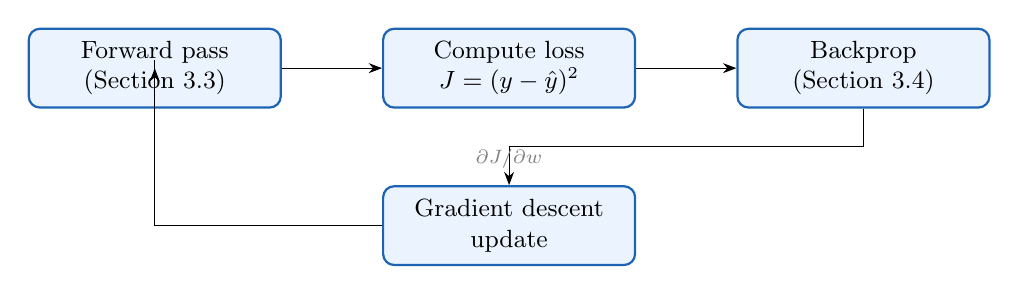
\begin{tikzpicture}[
  box/.style={draw=mainblue, fill=boxbg, rounded corners=4pt,
              minimum width=3.2cm, minimum height=1.0cm,
              font=\small, align=center, thick},
  >=Stealth
]
  \node[box] (fwd)  at (0,    0) {Forward pass\\(Section 3.3)};
  \node[box] (loss) at (4.5,  0) {Compute loss\\$J = (y-\yhat)^2$};
  \node[box] (bwd)  at (9.0,  0) {Backprop\\(Section 3.4)};
  \node[box] (upd)  at (4.5, -2) {Gradient descent\\update};

  \draw[->] (fwd)  -- (loss);
  \draw[->] (loss) -- (bwd);
  \draw[->] (bwd)  -- ++(0,-1) -| (upd);
  \draw[->] (upd)  -- ++(-4.5,0) |- (fwd);

  \node[font=\scriptsize, gray] at (4.5, -1.15) {$\partial J/\partial w$};
\end{tikzpicture}
\end{center}

\vspace{0.5em}

\begin{notebox}
\textbf{Coming next --- Section 3.5: Adam.}
Plain gradient descent works, but it can be slow or sensitive to the
learning rate.  Adam is a smarter update rule that adapts the step size for
each weight automatically.  We will see how it improves on plain gradient
descent with only a small change to the update formula.
\end{notebox}

\end{document}
